\cleardoublepage
\chapter{文献综述}
\section{引言} 
形变传感器的研究进展和趋势如何?
各类形变传感器各有何优缺点?
在各种应用场景下应使用哪一类形变传感器?
使用某类传感器时可以获得哪一类的数据?
如何通过不同类别的数据重建出曲线的空间各点坐标?
如何根据各点坐标渲染出3D图形?
又如何将服务端重建的点坐标安全又实时地传输到客户端渲染程序?

本章将基于各类研究与文献来讨论这些问题。

\section{国内外研究现状}
\subsection{形变传感器的研究方向及进展}

形变传感器主要分为两大类,一类是传统形变传感器(Conventional Shape Sensors, CSS),
另一类是光纤形变传感器(Fiber Optic Shape Sensors, FOSS), 
其中传统形变传感器又分为非接触式和接触式两种。

非接触式传感器包括视觉系统传感器(如相机)、
无线电监测与测距(Radio Detection and Ranging, RaDAR)
或光监测与测距(Light Detection and Ranging, LiDAR)传感器,
这些传感器的性能与正确性受环境温度和污染干扰很大。

随着传感器的需求场景越来越多且复杂,非接触传感系统越来越局限,
对小型且灵活的接触式传感器的需求也就越来越大。
接触式传感器可以直接连接到物体上随其移动,
并将位置转换为光、电信号以感测形状、曲率、弯曲和扭曲。

\subsubsection{接触式传统形变传感器}

接触式CSS主要分为电阻压力传感器、光电传感器和微机电系统(Micro-Electo-Mechanical System, MEMS)传感器。
它们各自的简介、优缺点和应用如下表\cite{recent-dev-in-foss}:

\begin{table}[!htbp]\small
\begin{center}
\begin{tabular}{p{0.20\textwidth}p{0.20\textwidth}p{0.30\textwidth}p{0.30\textwidth}}
\toprule
\textbf{传感器技术} & \textbf{简介} & \makebox[5cm][c]{\textbf{优点与应用}} & \makebox[5cm][c]{\textbf{缺点}}\\

\midrule

电阻压力传感器 & 用于短距离二维弯曲或关节运动测量。&
\begin{itemize}
\setlength{\itemsep}{0pt}
\setlength{\parsep}{0pt}
\setlength{\parskip}{0pt}
    \item 低成本;
    \item 与其它电器件相兼容;
    \item 非常适用于可穿戴电子产品。
\end{itemize}
& 
\begin{itemize}
\setlength{\itemsep}{0pt}
\setlength{\parsep}{0pt}
\setlength{\parskip}{0pt}
    \item 不够精准;
    \item 尺寸重量过大,不适用于小尺寸的自动控制应用;
    \item 复杂且接线繁琐,不适用于大规模应用。
\end{itemize} \\

\midrule

光电传感器 & 基于密集的传感器网络工作:一种可计算物体3D表面的算法解决方案;一种电阻率传感器网络;三轴陀螺仪、三轴加速 度计和航班时间距离传感器。&
\begin{itemize}
\setlength{\itemsep}{0pt}
\setlength{\parsep}{0pt}
\setlength{\parskip}{0pt}
    \item 作为可穿戴设备检测脊椎姿势变化,进行医疗运动和预防伤害方面具有巨大潜力;
    \item 易于大规模生产;
    \item 与Arduinos等价格低廉的微电子设备兼容。
\end{itemize}
& 
\begin{itemize}
\setlength{\itemsep}{0pt}
\setlength{\parsep}{0pt}
\setlength{\parskip}{0pt}
    \item 对于工业应用而言,不是可靠且准确的解决方案;
    \item 要求传感器周围有自由空间,以便光学传感器能够正常工作;
    \item 无法保证精度;
    \item 不够灵活。
\end{itemize} \\

\midrule

MEMS传感器 & 结合了加速度计、陀螺仪和磁力计的微电机系统。&
\begin{itemize}
\setlength{\itemsep}{0pt}
\setlength{\parsep}{0pt}
\setlength{\parskip}{0pt}
    \item 钻井;
    \item 地面监控;
    \item 远程测量;
    \item 适用于密闭空间;
    \item 精加工。
\end{itemize}
& 
\begin{itemize}
\setlength{\itemsep}{0pt}
\setlength{\parsep}{0pt}
\setlength{\parskip}{0pt}
    \item 难以定制;
    \item 笨重;
    \item 低柔韧性(长关节);
    \item 测量分辨率低;;
    \item 昂贵;
\end{itemize} \\
\bottomrule
\end{tabular}
\caption{接触式CSS的优缺点对比}
\end{center}
\end{table}

分析可知这三种 CSS 传感器各自的适用场景:

\begin{itemize}
    \item 电阻压力传感器适用于消费级电子产品,如游戏用压感器、心率检测仪等。
    \item 光电传感器适用于通用基础设备,如医疗运动用人体肌肉脊椎形状传感。
    \item MEMS传感器适用于大型工程,如钻井、海床监控等。
\end{itemize}

\subsubsection{光纤形变传感器}

光纤传感的出现让实时确定物体的形态成为了一个很有前景的研究方向。
FOSS利用光纤传感器(Fiber Optic Sensors, FOS)来实现相对位置测量,
或是使用嵌入式FOS实现物体形状的测量。
FOSS被设计用于定向应变测量,例如,
FOSS可以由三芯光纤布拉格光栅(Fiber Bragg Grating, FBG)传感器平面组成,
该传感器平面测量应变以进行对象的多维曲率计算,因此可以在计算机模型中用于重建对象的2D和3D形状。

通常,FOSS与CSS相比具有许多明显而实用的优点,例如:

\begin{itemize}
\item FOSS可以仅由一个远程询问器单元进行监控,而无需布线和连接许多传感器。
\item 传感器的位置不需要电力,因此可以将其放置在传统手段无法接近的地方,并测量这些部位的应变或弯曲。
\item 小尺寸的光纤(直径在100μm和2 mm之间)可以被嵌入非常薄的材料、表面、结构中,或者嵌入到杆或小型设备的中心。
\item 光纤传感器不受外部电磁场的影响。
\end{itemize}

FOS的发展趋势如下表\cite{recent-dev-in-foss}:

\begin{table}[!htbp]\small
\begin{center}
\begin{tabular}{p{0.20\textwidth}cp{0.80\textwidth}}
\toprule
\textbf{进展} & \textbf{年份} & \makebox[5cm][c]{\textbf{简介}}\\

\midrule

弯曲传感器 & \textasciitilde 1980 & 确定了三种主要的早期弯曲感测方法。它们分别是:
通过正常光纤传输的功率变化感测;
通过配备了弯曲调制器的光纤传输功率变化来感测;
通过同一包层中并行核心之间的串扰而导致的传输功率变化来感测。
\\
\\
定向弯曲传感器 & \textasciitilde 1990 & 通过使用多根单独的光纤和多芯光纤,可以检测光纤弯曲方向。
其采用了多种技术,如单个的FBG、宏弯曲调制器、多芯光子晶体光纤模场变化和弯曲引起的芯串扰。
\\
\\
分布式弯曲传感 & \textasciitilde 1996 & 通过多路复用,光纤能够通过FBG在多个位置检测应变。 
最初,只有波分和时分多路复用用于光纤形状感测,这限制了传感器的数量和最小的弯曲半径。
\\
\\
第一款商用3D光纤形变传感(ShapeTape)& \textasciitilde 1999 & ShapeTape是最早用于计算物体形状和表面的光纤3D测量设备之一。 
它是在1990年代基于光纤压力传感器开发的。 
由于价格高,范围、灵活性和准确性都很有限,ShapeTape在商业上并不成功。
\\
\\
基础光纤形变传感 & \textasciitilde 2000 & 通过多路复用检测多个位置处的弯曲,为三维形状感测提供了机会。
三个或更多芯的光纤提供了在多个位置检测方向应变的能力,从而可以重构空间中的光缆形状。
\\
\\
分布式光线形变传感 & \textasciitilde 2004 & 在多个磁芯上数千个应变位置的检测使连续光栅感测三维形状成为可能,
从而消除了先前形状感测技术的离散性质。 
光频域反射计(Optical Frequency Domain Reflectometry, OFDR)可以利用普通光纤和连续光栅光纤中的瑞利反向散射光进行形状感测。
\\
\\
用于工业和医疗机器人的光纤形变传感 & \textasciitilde 2006 & 各种专利的出现促使着工业和医疗器械中FOSS的使用,
这似乎是工业界第一次在实际应用中对FOSS表现出兴趣。
\\
\\
螺旋光纤布拉格光栅传感器 & \textasciitilde 2008 & 这篇论文似乎是对多芯光纤中使用螺旋FBG进行扭曲和弯曲测量的第一个演示,
这为如何基于FOSS实现完整的3D重建提供了重大改进思路。
\\
\\
光纤形变传感可视化 & \textasciitilde 2009 & 随着返回信号愈发复杂,渲染出使用光纤形状感测的电缆变得更具挑战性。
自2009年以来,越来越多的论文和专利概述了实时渲染FOSS输出的各种方法。
\\
\\
基于光纤形变传感器的力传感 & \textasciitilde 2013 & 使用光纤形状感测电缆测量力不仅可以检测光纤的位置,
还可以检测该点的力。这些论文和专利自2013年以来由医疗器械公司出版,
为多功能形状传感器开辟了道路。
\\
\\
基于多芯光纤和分布式FOSS的分布式布里渊散射 & \textasciitilde 2016 & 首次演示了通过多芯光纤(Multi-Core Fiber, MCF)
中偏心纤芯的布里渊频移来测量长光纤(1km)中的曲率,为远程形状感测带来了新的可能性。
\\
\\
螺旋多芯光纤中的连续光栅 & \textasciitilde 2017 & 关于连续光栅多芯光纤的研究有了新的进展。
复合多芯光纤的商业可用性对于开发高分辨率和分布式FOSS来说至关重要。
\\
\bottomrule
\end{tabular}
\caption{FOSS的发展趋势}
\end{center}
\end{table}

\subsection{曲线重建算法}
曲线重建主要分为两个部分,一个是连续化,即将离散的数据连续化;
另一部分是拟合,根据数据拟合得到绝对坐标系下的曲线各点坐标。
根据传感器的种类不同,所测得的数据类型不同,这两部工作的执行顺序也可以不同。

如MEMS惯性传感器主要测量加速度数据,并对加速度数据进行二次积分而得到测量点位移,
故可以在计算测量点坐标之后再进行连续化;而像FBG传感器所得到的是测量点的曲率数据,
难以直接计算获得该点坐标,必须先对曲率数据进行连续化,然后通过拟合算法计算得出各点的坐标。

本小结主要讨论连续化算法和基于曲率数据的曲线拟合算法。

\subsubsection{连续化算法}

常用的连续化算法有线性插值法、
贝塞尔(Bezier)曲线插值法、
B样条曲线插值法和三次样条曲线插值法。

\begin{enumerate}[label=(\Alph*)]
    \item \textbf{线性插值法} \\
    线性插值法即认为每两个测量点处的曲率变化是线性的,即:
    \begin{equation}
    \left\{
        \begin{array}{lr}
        k_{i, i+1} (S) = a_{i, i+1} (S - S_i) + k_i, \ S_i\leq S\leq S_{i+1}\\
    \\
        a_{i, i+1} = \frac{k_{i+1} - k_i}{S_{i+1} - S_i}
    \\
        k_0 = S_0 = 0
        \end{array}
    \right.
    \end{equation}

    线性插值算法简单,计算速度快;但是分割点连接处不平滑,跟实际产生的曲线可能存在一定的差距。

    \item \textbf{贝塞尔曲线插值法} \\
    贝塞尔曲线的一般式如下:

    \begin{equation}
        k(S) = \Sigma_{i=0}^nC_n ^ i a_i(1-S)^{n - i}S^i
    \end{equation}

    贝塞尔曲线插值结果很光滑,但存在另外的问题:

    \begin{enumerate}[label=(\alph*)]
        \item 确定了测量点数$n+1$,也就决定了所定义的Bezier曲线的阶次$n$,很不灵活。
        \item 当测量阶次$n$较大时,曲线的阶次将比较高。此时,测量点对曲线形状的控制将明显减弱。
        \item Bezier的调和函数$\Sigma_{i=0}^nC_n ^ i (1-S)^{n - i}S^i$的值在开区间$(0,1)$内均不为0。
        因此,所定义的曲线在$(0<S<1)$的区间内的任何一点均要受到全部顶点的影响,
        即改变其中任一个顶点的位置,都将对整条曲线产生影响,因此对曲线进行局部修改是不可能的。
    \end{enumerate}

    \item \textbf{B样条曲线插值法} \\
    为了克服以上提到的在Bezier曲线中存在的问题,
    Gordon、Riesenfeld和Forrest等人拓展了Bezier曲线,用n次B样条基函数替换了伯恩斯坦基函数,
    构造了B样条曲线。B样条曲线除了保持Bezier曲线所具有的优点外,还增加了可以对曲线进行局部修改这一突出的优点。
    除此之外,它还具有对特征多边形更逼近以及多项式阶次较低等优点。因此,B样条曲线在外形设计中得到了更广泛的重视和应用。

    \begin{equation}
    \left\{
        \begin{array}{lr}
        k(S) = \Sigma_{i=0}^n a_i B_{i, deg}(S)
    \\
        B_{i, deg}(S) = \frac{S-S_i}{S_{i+deg} - S_i}B_{i, deg-1}(S) +\frac{S_{i + deg +1}-S}{S_{i + deg +1} - S_i}B_{i+1, deg-1}(S) 
        \end{array}
    \right.
    \end{equation}

    上面就是B样条曲线的方程,其中$B(S)$被称为基础函数表,
    基础函数表本质上是个递归方程,同时也是一个中间参数。
    当前$deg$阶的元素需要通过两个$deg-1$阶的元素获得,
    $deg-1$阶的元素则需要通过$deg-2$阶的元素获得……以此类推,
    直到递归$deg$次以后,回退到0阶为止。

    但是,回退到0阶的时候怎么算呢?B样条算法规定,回退到0阶时使用以下公式: 

    \begin{equation}
    B_{i, 0} = \left\{
        \begin{array}{lr}
        1, \ S_i \le S \le S_{i+1}
    \\
        0, \ S \textless S_i \ or \ S \textgreater S_{i+1}
        \end{array}
    \right.
    \end{equation}

    B样条曲线克服了Bezier曲线遇到的问题,
    但其在多个离散曲率检测点的曲率数据不全在拟合出的曲率连续化曲线上,
    这会产生一定的拟合误差。我们可以采用三次样条曲线插值法来解决这个问题。

    \item \textbf{三次样条曲线插值法} \\
    假设曲率和弧长的关系为:

    \begin{equation}
        k(S) =  a_i + b_i (S - S_i) + c_i  (S - S_i)^2 + d_i (S - S_i)^3
    \end{equation}

    且曲线在第 i 个分割点满足方程:

    \begin{equation}
    \left\{
        \begin{array}{lr}
        k_i(S_i) = C_i
    \\
        k_i(S_{i+1}) = C_{i+1}
    \\
        k_i'(S_{i+1}) = k_{i+1}'(S_{i+1})
    \\
        k_i''(S_{i+1}) = k_{i+1}''(S_{i+1})
        \end{array}
    \right.
    \end{equation}

    即曲率原函数、一阶和二阶微分均满足连续性关系,这就能保证拟合出的曲率曲线是足够光滑的。

    再将此方程组与下式联立:

    \begin{equation}
    \left\{
        \begin{array}{lr}
        k(0) = 0
    \\
        k(S_n) = 0
        \end{array}
    \right.
    \end{equation}

    则可求得$a_i, b_i, c_i, d_i$四个系数的值,最终可通过曲线上每一个点距原点的弧长计算曲率。
\end{enumerate}

\subsubsection{拟合算法}

常用的拟合算法有曲率方向作为运动坐标系坐标轴的拟合算法和基于Frenet标架的拟合算法。

\begin{enumerate}[label=(\Alph*)]
    \item \textbf{曲率方向作为运动坐标系坐标轴的拟合算法} \\

    \begin{figure}
    \centering
    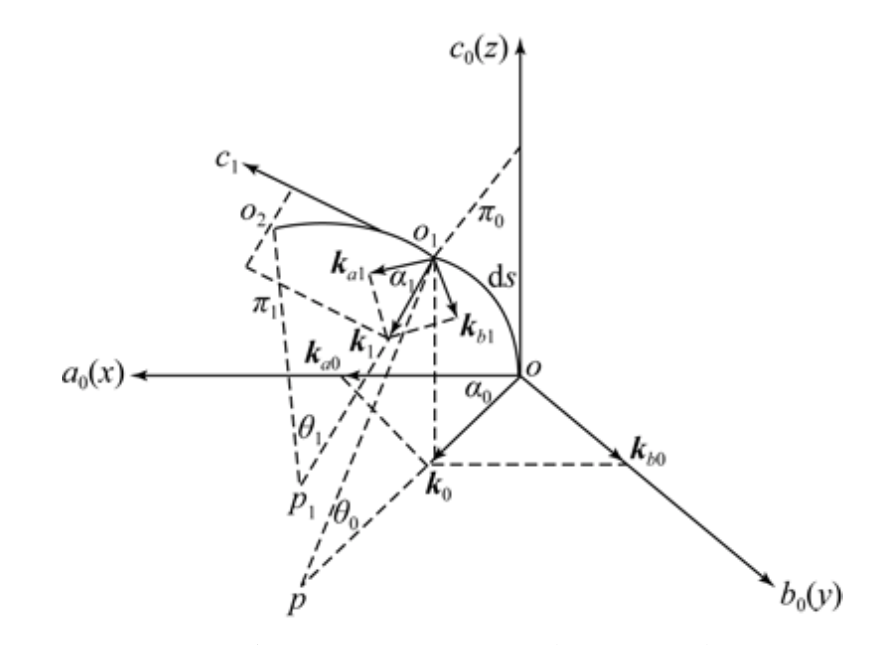
\includegraphics[scale=0.4]{cartesian-coordinate-system.png}
    \caption{曲率方向作为运动坐标系坐标轴}
    \end{figure}

    此算法的原理是以每个微段的方向为z轴建立运动坐标系$o_i-a_ib_ic_i$,
    并通过几何方法求得下一个点在此坐标系下的相对坐标$o_{i+1} \{d_{ai}, d_{bi}, d_{ci}\}$,
    再通过线性变换得到下一个点的运动坐标系$o_{i+1}-a_{i+1}b_{i+1} c_{i+1}$。
    这样就可以求得每个点在上个运动坐标系下的相对坐标以及当前坐标系相对上个坐标系的变换矩阵$t_{i, i+1}$。

    \begin{align}
        k_i &= \sqrt{k_{ai} ^ 2 + k_{bi} ^ 2}, \\
        \theta_i &= k_i \cdot d_s, \\
        cos\alpha_i &= k_{ai} / k_i, \\
        sin\alpha_i &= k_{bi} / k_i, \\
        d_a &= \frac{cos\alpha_i \cdot (1 - cos\theta_i)}{k_i}, \\
        d_b &= \frac{sin\alpha_i \cdot (1 - cos\theta_i)}{k_i}, \\
        d_c &= \frac{sin\theta}{k_i}, \\
        t_{i, i+1} &= \left[
            \begin{matrix}
                cos \alpha_i & -sin \alpha_i & 0 \\
                sin \alpha_i & cos \alpha_i & 0 \\
                0 & 0 & 1
            \end{matrix}
            \right]
            \cdot
            \left[
            \begin{matrix}
                cos \theta_i & 0 & sin \theta_i \\
                0 & 1 & 0 \\
                -sin \theta_i & 0 & cos \theta_i \\
            \end{matrix}
            \right]
            \cdot
            \left[
            \begin{matrix}
                cos \alpha_i & sin \alpha_i & 0 \\
                -sin \alpha_i & cos \alpha_i & 0 \\
                0 & 0 & 1
            \end{matrix}
            \right]
    \end{align}

    当前坐标系点乘三个矩阵的几何意义分别为:\\
    \begin{enumerate}
        \item 绕$\vec c_i$旋转一个$\alpha_i$角使得$\vec a_i$与$\vec k_i$同向;
        \item 绕$\vec b_i$旋转一个$\theta_i$角得到$\vec c_{i+1}$;
        \item 绕$\vec c_{i+1}$旋转一个$-\alpha_i$角得到$\vec a_{i+1}$和$\vec b_{i+1}$。
    \end{enumerate}

    将变换矩阵累乘即可得到各运动坐标系相对绝对(原点)坐标系的变换矩阵 $T_i$。
    然后将相对坐标$o_{i+1} \{d_{ai}, d_{bi}, d_{ci}\}$乘以$T_i$的逆矩阵即可得绝对坐标。

    \item \textbf{基于Frenet标架的拟合算法} \\
    我们也可以使用微分几何中常用的Frenet坐标标架。令$\vec T$为切向量,$\vec N$为主法向量,指向微段方向;$\vec B$为副法向量,
    则有:$\vec B = \vec T \times \vec N$。

    假设第$i$段曲线在$xoz$平面内,则两端点平移量$p_{i+1}$有:
    \begin{equation}
        p_{i+1} = [-(1-cos \ \theta_i)/k_i \quad 0 \quad sin \ \theta_i/k_i]^T
    \end{equation}
    曲率$k_i$、弧长$d_s$和弧角$\theta_i$满足$\theta_i = d_s \cdot k_i$。坐标系平移后沿$B_i$轴旋转$\theta_i$,则有:
    \begin{equation}
    [T_{B_i} ^ {\theta_i}] = \left[
        \begin{matrix}
        cos \theta_i & 0 & -sin \theta_i & 0 \\
        0 &1 & 0 & 0 \\
        sin \theta_i & 0 & cos \theta_i & 0 \\
        0 & 0 & 0 & 1 \\
        \end{matrix}
    \right]
    \end{equation}
    接着将坐标系沿$T_i$旋转$\Delta \phi_{i+1}$,其值由下式求出:
    \begin{equation}
    \Delta \phi_{i+1} = \begin{cases}
        \phi_{i+1} - \phi_i,&(\phi_{i+1} \ge \phi_i) \\
        2\pi + \phi_{i+1} - \phi_i,&(\phi_{i+1} \textless \phi_i)\\
    \end{cases}
    \end{equation}
    则有:
    \begin{equation}
    [T_{T_i} ^ {\Delta\phi_{i+1}}] = \left[
        \begin{matrix}
        cos \Delta\phi_{i+1} & -sin \Delta\phi_{i+1} & 0 & 0 \\
        sin \Delta\phi_{i+1} & cos \Delta\phi_{i+1} & 0 & 0 \\
        0 & 0 & 1 & 0 \\
        0 & 0 & 0 & 1 \\
        \end{matrix}
    \right]
    \end{equation}
    由此可求得一个微段运动坐标系的变换矩阵:
    \begin{equation}
    [t_{i+1}] = \left[
        \begin{matrix}
        & [T_{i+1}] & & p_{i+1} \\
        0 & 0 & 0 & 1 \\
        \end{matrix}
    \right]
    \end{equation}
    其中$[T_{i+1}] = [T_{B_i} ^ {\theta_i}] \cdot [T_{T_i} ^ {\Delta\phi_{i+1}}]$。

    通过此变换矩阵即可求得每个点的运动坐标系和下个点的相对坐标,再通过变换矩阵的逆矩阵求得绝对坐标,最终拟合出曲线。

\end{enumerate}

\subsection{三维渲染技术}

三维渲染是通过电脑计算的方式把模型从三维模型网格呈现出二维真实感高的图像,
计算过程包含光线及辅助光线、材料的材质和纹理、相机相关设置等综合变量。

三维渲染包括实时渲染和非实时渲染。

实时渲染主要应用在游戏领域,电脑会实时的计算和展示所渲染的结果,帧率在20-120左右。
因此需要在帧率一定的情况下最大化渲染的真实性。计算机在图像处理的过程中会用到一些“技巧”以迎合肉眼感官,
这些“技巧”包括镜头光晕(lends flare)、景深(depth of field)和动态模糊(motion blur)等。
计算机的算力决定了渲染的真实感,通常需要GPU来协助完成。

非实时渲染通常是电影或视频,借助计算机有限的算力,通过延长渲染时间达到更加真实的效果。
射线追踪(ray tracing)和辐射度算法(radiosity)是非实时渲染常用的技巧,以达到更加真实的感觉。
随着技术的发展,不同种类的物质形式有了更精确的计算技巧,
例如粒子系统(模拟雨、烟和火)、容积取样(模拟雾、灰尘)、焦散性质和子面散射(subsurface scattering)。
渲染过程中把不同层的物质分开计算后合成一个最终布景。

本小结主要介绍实时渲染中常用的技术。

\subsubsection{OpenGL}

OpenGL(Open Graphics Library)是一种用于渲染2D或3D图像的跨平台编程接口,
它并不指任何一种特定实现,而是一种接口规范。与之类似的还有仅用于Windows平台的Direct3D。

OpenGL由Khronos Group开发维护,GPU的硬件开发商则需要提供满足OpenGL规范的驱动程序,
它们负责将OpenGL定义的API命令翻译为GPU指令。

这个接口由近350个不同的函数调用组成,用来从简单的图形数据绘制复杂的三维图像,
常用于CAD、虚拟现实、科学可视化程序和电子游戏开发。 

它有很多的具体实现和编程语言绑定,如JavaScript绑定的WebGL;
C绑定的WGL、GLX和CGL;iOS提供的C绑定;Android提供的Java和C绑定。

\subsubsection{WebGL和Three.js}

WebGL是浏览器上的OpenGL实现,用于在任何兼容的Web浏览器中呈现交互式3D和2D图形。
WebGL通过引入一个与OpenGL ES 2.0紧密相符合的API,可以在HTML5 <canvas>元素中使用。

目前支持WebGL的浏览器有:Firefox 4+、Google Chrome 9+、Opera 12+、Safari 5.1+和Internet Explorer 11+;
但是WebGL一些特性也需要用户的硬件设备支持。

WebGL几乎是完全地“跨平台”,使用任何支持WebGL的浏览器打开网页即可完成客户端渲染,而无需下载另外的软件或浏览器插件。

Three.js是一个基于WebGL的3D图形库,它封装了很多实用的图形组件。由Ricardo Cabello在2010四月于GitHub首次发布。
它的起源可以追溯到他在本世纪初演示场景的参与。代码最初使用ActionScript,稍后2009年移植到JavaScript。在Cabello看来,
转移到JavaScript有两个优点:每次运行前没有编译代码和平台独立性。
随着WebGL的到来,Paul Brunt增加渲染功能,这使得Three.js设计与绘制的代码成为一个模块,而不是核心本身。
它提供了如下功能:

\begin{itemize}
    \item 效果:浮雕,对眼和视差屏障;
    \item 场景:在运行时添加和删除对象、雾;
    \item 镜头:视角和正字法;控制器:轨迹球、FPS、路径等;
    \item 动画:电枢、运动学、逆运动学、变形和关键帧;
    \item 灯光:环境、方向、点和点光;阴影:投射和接收;
    \item 材料:Lambert、海防、光滑阴影等;
    \item 材质:访问完整的OpenGL着色语言(GLSL)能力:镜头光晕;
    \item 对象:网格、粒子、精灵、线、带、骨头等;
    \item 几何:平面、立方体、球体、圆环、3D文本等;修改器:车床、挤压和管;
    \item 数据加载器:二进制、图像、JSON和场景;
    \item 事业:全套时间和三维数学函数包括锥、矩阵、四元、UVs等;
    \item 输入输出:与three.js兼容的 JSON文件:Blender、openctm、FBX、Max,OBJ;
    \item 支持:API文档持续更新,公共论坛和维基全面运作;
    \item 例子:超过150个文件的编码例子加字体、模型、纹理、声音和其他支持文件;
    \item 调试:Stats.js、WebGL检查器、Three.js检查器。
\end{itemize}
另外Three.js依据MIT公用许可证发布,完全开源开放,且可以在所有支持WebGL 1.0的浏览器中运行。

\subsection{网络数据传输技术}

计算机网络模型一般指OSI七层模型,有时也使用TCP/IP四层模型。
本小结主要介绍常用的应用层协议(OSI模型中的会话层、表示层和应用层;TCP/IP模型中的应用层)。

\subsubsection{HTTP}

超文本传输协议(Hyper-Text Transfer Protocol, HTTP)是一个用于传输超媒体文档(例如 HTML)的应用层协议。
它是为Web浏览器与Web服务器之间的通信而设计的,但也可以用于其他目的。
HTTP遵循经典的客户端-服务端模型,客户端打开一个连接以发出请求,然后等待它收到服务器端响应。
HTTP是无状态协议,这意味着服务器不会在两个请求之间保留任何数据(状态)。
该协议虽然通常基于传输控制协议(Transmission Control Protocol, TCP),但可以在任何可靠的传输层上使用。

HTTP协议目前有1.0,1.1和2.0三个版本,前两个版本是包结构兼容的文本协议;而HTTP/2则是二进制协议,不与HTTP/1.x兼容。

目前使用最广泛的版本是HTTP/1.1。另外,HTTP/1.x协议提供了一种特殊的机制,
这一机制允许将一个已建立的连接升级成新的、不相容的协议。通常来说这一机制总是由客户端发起的
(不过也有例外,比如说可以由服务端发起升级到传输层安全协议(Transport Layer Security, TLS)),
服务端可以选择是否要升级到新协议。借助这一技术,连接可以以常用的协议启动(如HTTP/1.1),
随后再升级到HTTP/2甚至是WebSocket。

\subsubsection{WebSocket}

WebSocket(简称WS)是浏览器提供的一种浏览器与服务器进行全双工通讯的网络技术,
它是一个独立的协议,但支持使用HTTP/1.x握手。

相比于HTTP/1.x,它有如下优点:

\begin{itemize}
    \item 支持双向通信,实时性更强;
    \item 更好的二进制支持;
    \item 较少的控制开销。连接创建后,WS客户端、服务端进行数据交换时,协议控制的数据包头部较小。在不包含头部的情况下,服务端到客户端的包头只有2~10字节(取决于数据包长度),客户端到服务端的的话,需要加上额外的4字节的掩码。而HTTP/1.x每次通信都需要携带完整的头部;
    \item 支持扩展。WS协议定义了扩展,用户可以扩展协议,或者实现自定义的子协议(比如支持自定义压缩算法等)。
\end{itemize}

其握手过程如下:

\begin{enumerate}
    \item 客户端发起升级协议请求(基于HTTP/1.x)\\
        \begin{lstlisting}
GET / HTTP/1.1 
Host: localhost:8080 
Connection: Upgrade 
Upgrade: websocket 
Sec-WebSocket-Version: 13 
Sec-WebSocket-Key: w4v7O6xFTi36lq3RNcgctw==
        \end{lstlisting}
        其中\fira{Sec-WebSocket-Version}不得低于13,\fira{Sec-WebSocket-Key}是一个随机字符串,用于防止无意的连接。
    \item 服务端协议升级响应 \\
        \begin{lstlisting}
HTTP/1.1 101 Switching Protocols
Connection: Upgrade
Upgrade: websocket
Sec-WebSocket-Accept: Oy4NRAQ13jhfONC7bP8dTKb4PTU=
        \end{lstlisting}
        其中\fira{Sec-WebSocket-Accept}由请求中的\fira{Sec-WebSocket-Key}生成,
        用于客户端校验;如果客户端校验无误,则WS握手成功。
\end{enumerate}

\subsubsection{gRPC}

gRPC协议是一种由Google制定的远程过程调用(Remote Procedure Call, RPC)协议,
其基于HTTP/2.0和Protocol Buffers,故获得了以下特性:

\begin{itemize}
    \item 支持客户端双向流(由客户端发起)和服务器端流(由服务器发起);
    \item 高效的传输和解析性能(二进制协议,帧数据);
    \item 高连接利用率(HTTP/2通过数据帧支持了连接的多路复用);
    \item 支持流控;
    \item 高效且稳健(支持向后兼任)的序列化、反序列化(由Protocol Buffers提供);
    \item 支持各种主流编程语言(Google提供一个grpc-core C库供原生语言绑定;同时提供grpc-web供浏览器使用)。
\end{itemize}

\subsubsection{TLS}

TCP是明文传输且无验证机制的,其存在三大风险:

\begin{enumerate}
    \item 窃听风险(eavesdropping):第三方可以获知通信内容;
    \item 篡改风险(tampering):第三方可以修改通信内容;
    \item 冒充风险(pretending):第三方可以冒充他人身份参与通信(中间人攻击)。
\end{enumerate}

TLS是为了解决这三大风险而设计的,其设计目标是:

\begin{enumerate}
    \item 所有信息都是加密传播,第三方无法窃听;
    \item 具有校验机制,一旦被篡改,通信双方会立刻发现;
    \item 配备身份证书,防止身份被冒充。
\end{enumerate}

1994年,NetScape公司设计了SSL(Secure Sockets Layer)协议的1.0版,
但是未发布。次年,NetScape公司发布SSL2.0,但很快发现有严重漏洞。
1996年,SSL3.0版问世,得到大规模应用。

直到1999年,互联网协会ISOC接替NetScape公司发布了SSL的升级版TLS1.0。
2006年和2008年,TLS进行了两次升级,分别为TLS1.1版和TLS1.2。
最新的变动是2018年发布的TLS1.3标准提案。

TLS是介于TCP协议和上层应用协议之间的安全层,其作用机理是基于TCP连接建立安全的TLS连接,
再基于TLS连接实现上层协议。
其建立安全连接的基本思路是采用公钥加密法;也就是说,客户端先向服务器端索要公钥,
然后用公钥加密信息;服务器收到密文后,用自己的私钥解密。

基于RSA密钥交换算法的TLS连接建立大致流程如下:

\begin{enumerate}
    \item 客户端发起连接请求,服务器返回公钥和证书;
    \item 客户端验证证书可信后生成用于对称加密的“对话密钥”,并使用服务器端返回的公钥加密该密钥,将密文发给服务器端;
    \item 服务器使用私钥解密得到“对话密钥”,之后双方使用该对话密钥对信息加密。
\end{enumerate}

其中证书由各权威组织发行,用于保证公钥没有被篡改,故可杜绝中间人攻击。
基于公私钥的非对称加密计算量很大,故只用于加密传递“对话密钥”,之后通过“对话密钥”对信息进行快速对称加密。

基于TLS的应用层协议都会在原本的协议名后加一个 “S”,如HTTPS、FTPS等,表示此连接是安全的。

\section{研究展望}

传感器领域,在实时性、准确度要求不是很高且测量环境允许的场景下,
CSS具有成熟的产业链和颇具规模的市场,且表现不出特别的劣势。
但在高实时性、准确性要求和恶劣环境(如电磁干扰、深水)下,FOSS表现出了压倒性的优势。
近年来FOSS在大范围、分布式传感的研究也获得了不错的进展,未来有望传感更大范围、高精度、多维度的实时信息。

连续化算法方面,线性插值简单快速但不平滑;
贝塞尔曲线平滑但随着测量点数量的上升复杂度急剧上升;
B样条曲线和三次样条曲率插值法则各有取舍。
其中B样条曲线平滑、通用易于编程实现,但在测量点过多的情况下可能不过测量点,导致拟合出的曲线与实际曲线有一定偏差;
三次样条曲率插值牺牲了一定的平滑度和编程简易度,换取了更高的准确性(曲线必过测量点)。

拟合算法方面,曲率方向作为运动坐标系坐标轴的拟合算法和基于Frenet架标的拟合算法实际上是同一种原理在两种架标下的解释,
本质上都是通过运动坐标系计算点的相对坐标,再通过变换矩阵求绝对坐标。但Frenet架标下少一次旋转操作,即可以减少一次矩阵运算。

3D渲染方面,随着WebGL技术的逐步成熟,使用浏览器做实时渲染已是时代的大势所趋,
渲染程序可以通过浏览器完美地跨平台并迅速地分发到世界各地。

网络数据传输方面,基于TLS的全双工流式通信协议(如 WSS (WebSocketS)和 H2 (HTTP/2 over TLS))逐渐成熟,
使得数据交互更加地快捷高效且安全。通过一台Web服务器,用户即使在地球另一端也可以使用任意浏览器获得数据,
甚至基于WebGL来获得实时的图像。

\newpage
\printbibliography[title={参考文献}]
